\documentclass[11pt,border=5pt]{standalone}
\usepackage{fontspec}
\setmainfont{cmunrm.otf}[BoldFont=cmunbx.otf,ItalicFont=cmunti.otf,BoldItalicFont=cmunbi.otf]
\usepackage{amsmath}
\usepackage{unicode-math}
\setmathfont{NewCMMath-Regular.otf}
\usepackage{tikz}
\usetikzlibrary{arrows.meta,patterns,angles,quotes}
\begin{document}
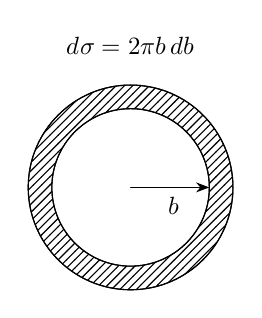
\begin{tikzpicture}[>=Stealth,font=\small,line cap=round,line join=round]
\draw (0,0) circle (1);\draw (0,0) circle (1.3);\draw[pattern=north east lines,even odd rule] (0,0) circle (1.3) (0,0) circle (1);
\draw[->,thin] (0,0) -- (1,0) node[pos=0.55,below] {$b$};
\node at (0,1.8) {$d\sigma=2\pi b\,db$};

\end{tikzpicture}
\end{document}
